\chapter{Reconhecimento de padrões}
Todo o processo, desde a organização dos dados até a etapa de classificação, foi implementado utilizando a linguagem de programação Java. A implementação foi feita em módulos, organizados da seguinte forma: Módulo organizador de dados, Módulo de geração de classificadores, Módulo de classificação, Módulo validador. No módulo organizador de dados os conjutnos de dados são organizados em subgrupos, cada subgrupo contendo vetores de todos os padrões, essa organização é importante para a etapa de validação do método. No Módulo de geração de classificadores está implementado o modelo de programação linear e são gerados os hiperplanos separadores. Os Módulos de classificação e validador são utlizados na etapa de teste, o primeiro realiza a classificação de de um vetor em um dos padrões separados pelo hiperplano e o segundo realiza a validação do método de reconhecimento de padrões utlizando o método cross validation.

Na figura \ref{img:diagrama_modulos} estão representadas as principais etapas realizadas durante os experimentos computacionais.

\begin{center}
	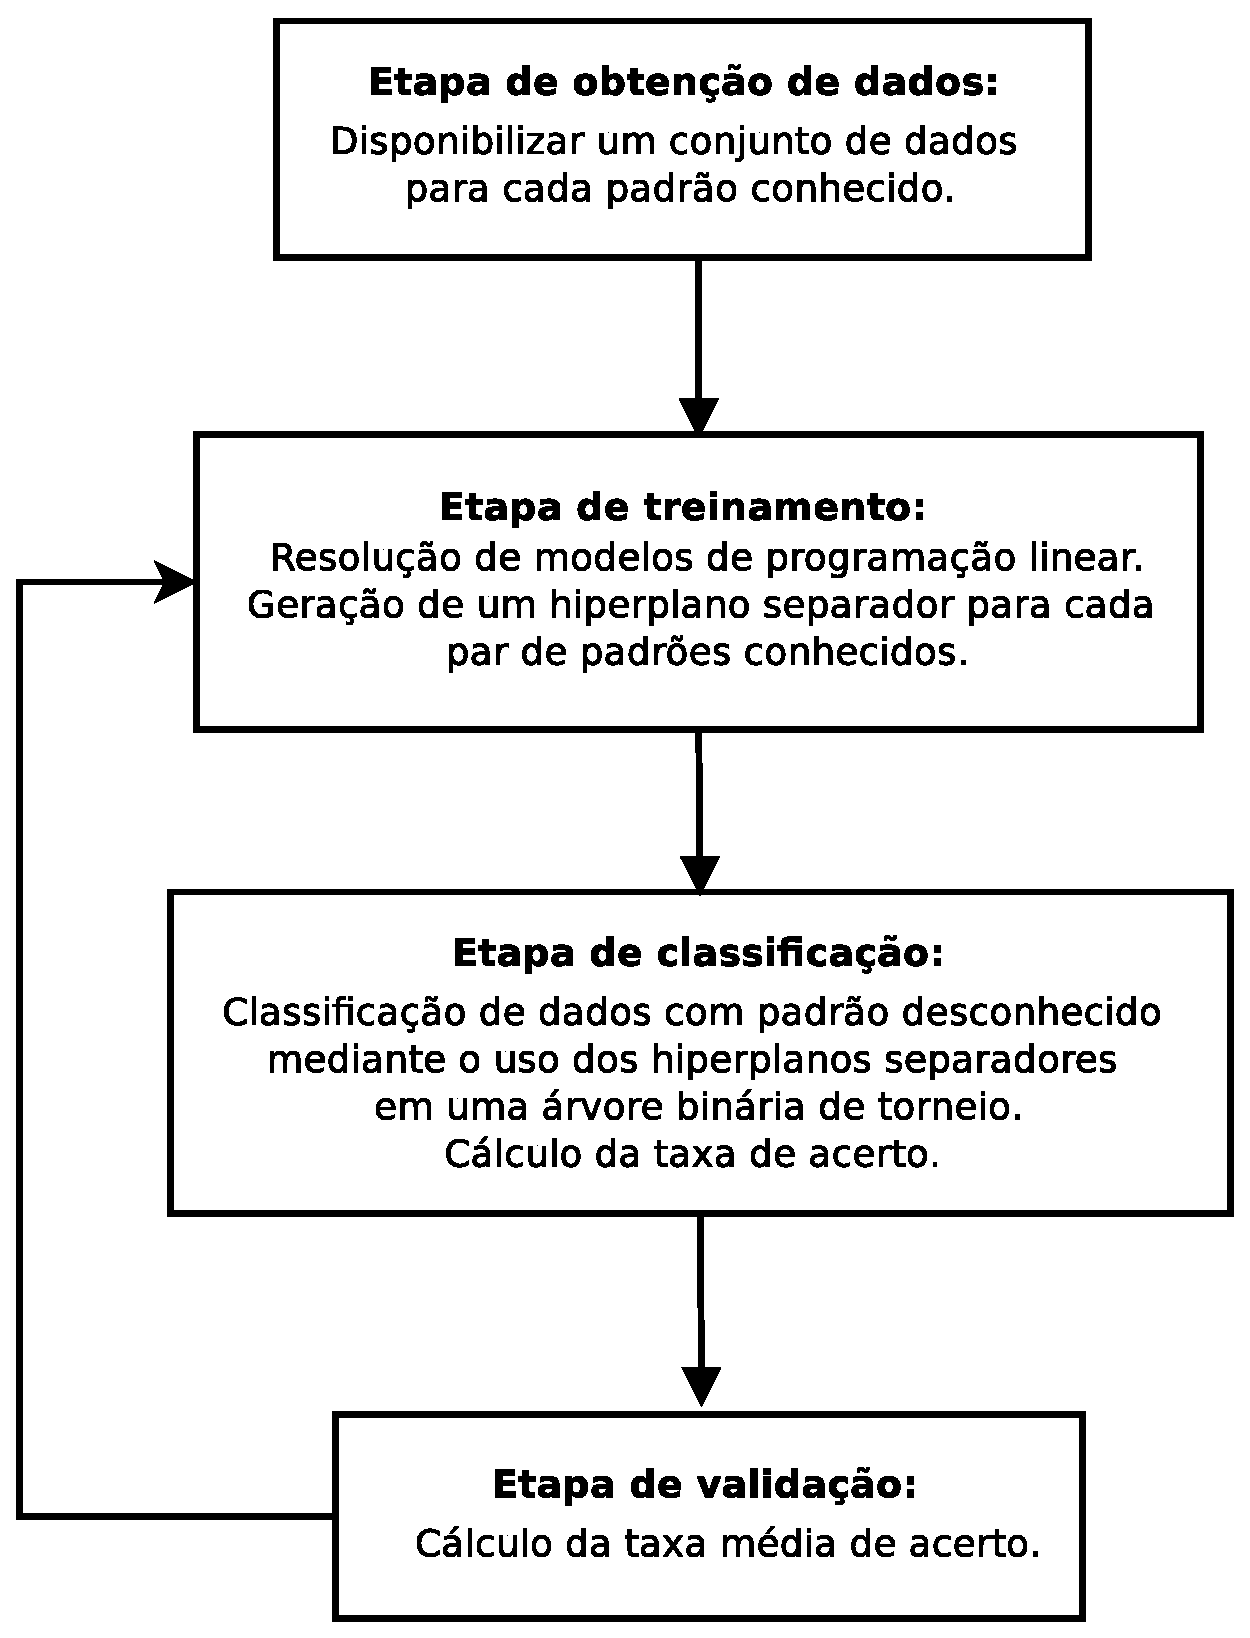
\includegraphics[scale=0.5]{graficos/diagrama_metodologia}
	\captionof{figure}{Diagrama das etapas realizadas nos experimentos}
	\label{img:diagrama_modulos}
\end{center}

Primeiramente os dados foram obtidos já no formato de vetores de caracteríticas ou extraídos de imagens, e depois foram divididos em subgrupos. Em seguida foram submetidos ao modelo de Programação Linear, reponsável por gerar os classificadores e por último vetores com padrão desconhecido foram classificados. As duas últimas etapas são repetidas a cada ciclo de teste, essas repetições são controladas pelo Módulo validador. Nas seções seguintes essas etapas serão apresentadas de forma mais detalhada.

\section{Etapa de obtenção de dados}
Nessa etapa inicial é obtido um conjuto de dados com um número de padrões \textit{p} conhecido. Um conjunto de dados com \textit{p} subconjuntos, um para cada padrão, onde cada subconjunto é composto por vetores contendo \textit{n} características. Para o reconhecimento de padrões, o número \textit{p} de padrões deve ser previamente conhecido, assim como o número de vetores de características para cada padrão.

\section{Etapa de treinamento}
Na tarefa onde o obejtivo é a separação de dois ou mais conjuntos de pontos, sendo que cada conjunto representa um padrão, busca-se um método para que essa separação seja obtida com resultado ótimo. Cada conjunto é o resultado de um conjunto de pontos e cada ponto é representado por um vetor de características.
Em \cite{Bennett92robustlinear} é proposto um modelo de programação linear capaz de um gerar um hiperplano, que separa dois conjuntos de pontos, minimizando a soma das violações dos pontos que permaneceram do lado "errado" do hiperplano. Dessa forma o modelo é capaz de gerar um hiperplano separador para pontos linearmente separáveis e para conjuntos linearmente inseparáveis, o modelo gera o melhor hiperplano de forma que essa média calculada seja mínima. Na figura abaixo estão ilustrados os casos de dois conjuntos linearmente separáveis e dois conjuntos linearmente inseparáveis.
 
\begin{figure}[!h]
\centering
\subfigure[]{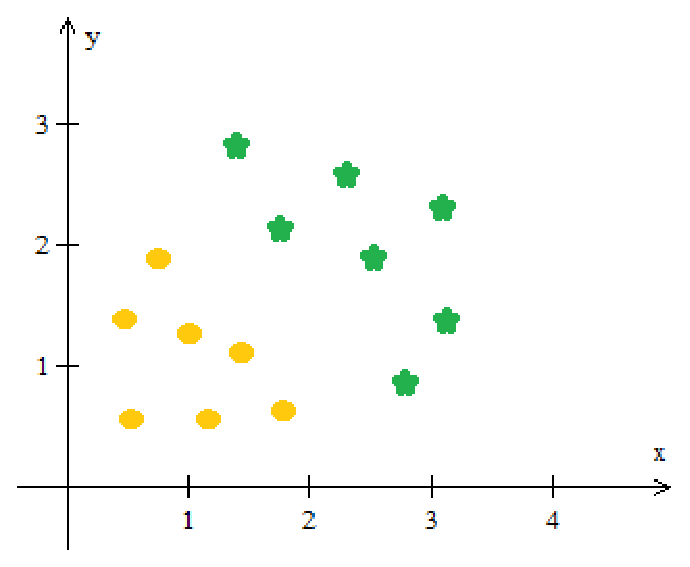
\includegraphics[scale=0.5]{graficos/linear_sepa}\label{fig1}}
\qquad
\subfigure[]{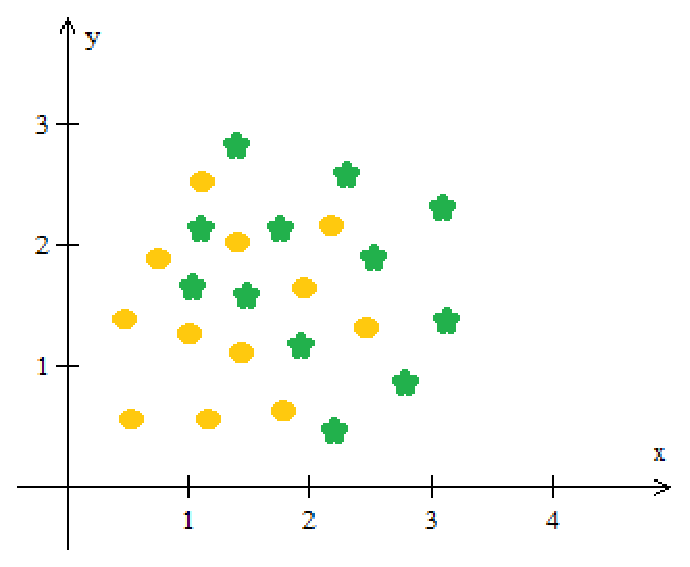
\includegraphics[scale=0.5]{graficos/linear_insepa}\label{fig2}}
\label{img:linear_sepa}
\caption{Em \ref{fig1} são apresentados dois conjuntos linearmente separáveis e em \ref{fig2} são apresentados dois conjuntos linearmente inseparáveis}
\end{figure}

É possível observar que na figura \ref{fig1} podem ser tratadas inúmeras retas seprando os dois conjuntos de pontos. Já na figura \ref{fig2} o modelo de programação linear poderá definir a melhor reta possível para separar os pontos.

A proposta do modelo e separa dois conjuntos de pontos, porém também pode ser utlizado em problemas onde busca-se a separação de múltiplos padrões. O presente trabalho foca nessa última abordagem, em todos os testes realizados o número de conjutnso de pontos é igual ou maior que três.

\subsection{O modelo}
Considerando dois conjuntos, no espaço n-dimensional $ R^{n} $, sendo o conjunto A representado pela matriz m x n, e o conjunto B representado pela matriz k x n. Contextualizando, k e m são as quantidades de pontos em cada conjunto, sendo que cada vetor de características é um ponto e n é a quantidade de características. O modelo gera um hiperplano que separa os pontos dos dois conjuntos. De forma que os m pontos do conjunto A fiquem de um lado do hiperplano e os k pontos do conjunto B fiquem do outro lado do hiperplano. Na figura abaixo o modelo é apresentado. E a seguir é apresentado de forma mais detalhada.

$$\min_{\omega ,\gamma ,y,z}\frac{e^{T}y}{m}+\frac{e^{T}z}{k}$$
$$s.a.\left\{\begin{matrix}-A\omega +e\gamma+e\leq y\\B\omega -e\gamma+e\leq  z\\ y\geq 0,y\geq 0\end{matrix}\right.$$

O modelo determina o hiperplano:
$$ x\omega = \gamma $$
Onde,  é $\omega$ o vetor normal ao hiperplano e $\gamma$ é um escalar. De forma que:
$$A\omega \geq e\gamma$$
e
$$B\omega \leq e\gamma$$
Onde e é um vetor de 1’s com dimensão m para o conjunto A e k para o conjunto B.
Para conjuntos linearmente separáveis torna-se fácil traçar um hiperplano separador, porém para conjuntos linearmente inseparáveis é necessária uma estratégia para que o hiperplano separador seja ótimo, nesse caso a estratégia utilizada é a minimização da soma das médias das violações dos pontos localizados do lado "errado" do hiperplano.
O modelo busca o melhor hiperplano, para isso gera dois hiperplanos limites somando ou subtraindo 1 unidade a equação do hiperplano separador:
$$A\omega \geq e\gamma + e$$
e
$$B\omega \leq e\gamma - e$$
De forma que o hiperplano separador fica localizado exatamente entre esses dois hiperplanos que formam uma faixa limite.
Detalhando o modelo de acordo com \citeonline{Eberson10LPseparaPontos}, considerando x como um vetor em $ R^{n} $, definimos:

$1.\ \ (x_{i})_{+} = \max_{i=1,2,...,n}{\left \{x_{i},0  \right \}}$

$2.\ \ \left \| xx \right \|_{1} = \sum_{i=1}^{n}\left | x_{i} \right |$

Podemos escrever o problema de minimização com norma da seguinte forma:

$$\min_{\omega ,\gamma }\frac{1}{m}\left \| \left ( -A\omega + e\gamma  + e \right )_{+} \right \|_{1} + \frac{1}{k}\left \| \left ( B\omega - e\gamma + e  \right )_{+} \right \|_{1}$$

Seja $g:R^{n} \mapsto R^{m} , h:R^{n} \mapsto R^{k}$ e S um subconjunto de $R^{n}$ . Os problemas abaixo possuem soluções idênticas:

$$\min_{x\in S}\left \| g(x)_{+} \right \|_{1} + \left \| h(x)_{+} \right \|_{1}$$


$$\min_{x\in S} e^{t}y + e^{t}z\\$$
$$ s.a.\left\{\begin{matrix}y\geq g(x)\\ z\geq h(x)\\ y\geq 0, z\geq0\end{matrix}\right.$$

Como $g(x)_{+}\geq g(x)$ e $h(x)_{+}\geq h(x)$ podemos observar que os valores ótimos de y e z podem der dados pelas igualdades $y=g(x)_{+}$ e $z=h(x)_{+}$.

A partir do problema de minimização temos o problema de programação linear equivalente:

$\min_{\omega ,\gamma ,y,z}\frac{e^{T}y}{m}+\frac{e^{T}z}{k} \; \; \; \; (a)\\
s.a.\left\{\begin{matrix}-A\omega +e\gamma+e\leq y\; \; (b)\\B\omega -e\gamma+e\leq  z\; \; (c)\\ y\geq 0,y\geq 0\; \; (d)\end{matrix}\right.$

\underline{Dados do Modelo}:
\begin{itemize}
\item{m}: quantidade de vetores de características correspondente ao primeiro padrão;
\item{k}: quantidade de vetores de características correspondente ao segundo padrão;
\item{A}: Matriz contendo o conjunto de vetores de caraterísticas do primeiro padrão;
\item{B}: Matriz contendo o conjunto de vetores de caraterísticas do segundo padrão;
\item{e}: vetor coluna unitário;
\end{itemize}

\underline{Variáveis do Modelo}:
\begin{itemize}
\item{$\omega$}: coeficientes do hiperplano que separa os conjuntos de pontos dos dois padrões;
\item{$\gamma$}: constante do hiperplano que separa os conjuntos de pontos dos dois padrões;
\item{y}: vetor contendo o quanto um ponto violou ;
\item{z}: vetor contendo as distâncias de cada imagem do conjunto B ao hiperplano separador mais um.
\end{itemize}

\underline{Formulação Matemática}:
A função objetivo (a) procura minimizar a soma das médias das violações dos pontos de ambos conjuntos. A restrição (b) exige que os pontos se encontrem necessariamente abaixo do hiperplano separador mais uma constante unitária.  A restrição (c) é análoga a restrição (b) aplicada ao segundo padrão. As equações em (d) definem a natureza das variáveis do modelo, como sendo não negativas.

\subsection{Exemplo Ilustrativo do Modelo Classificador}
Para ilustrar o modelo vamos considerar dois exemplos em $R^{2}$ \cite{Bennett92robustlinear} de forma que a ilustração gráfica fique mais facilmente compreensível.
\begin{itemize}
\item Exemplo1:

Considerando as matrizes a seguir:
$$A=\begin{bmatrix}1 & 1\\ 1 & 2\\ 1 & 3\\ 2 & 1\\ 2 & 2\\ 2 & 3\\ 2 & 4\\ 3 & 3\\ 3 & 4\end{bmatrix}
B=\begin{bmatrix}4 & 1\\ 4 & 2\\ 4 & 3\\ 5 & 2\\ 5 & 3\\ 5 & 4\\ 6 & 2\end{bmatrix}$$

Nesse caso, temos: m = 9 (quantidade de pontos da matriz A) e k = 7 (quantidade de pontos da matriz B).  Submetendo as matrizes ao modelo temos:
\begin{itemize}
\item[$\ast$] Valor da função objetivo = 0
\item[$\ast$] $\omega$ = [-2  0]
\item[$\ast$] $\gamma$ = -7
\item[$\ast$] y = [0 0 0 0 0 0 0 0 0]
\item[$\ast$] z = [0 0 0 0 0 0 0]
\end{itemize}
Como o valor da função objetivo depende dos vetores y e z, podemos notar que o valor 0 indica que os conjuntos A e B são linearmente separáveis. A seguir é apresentada a representação gráfica dos pontos e das retas geradas pelo modelo.

\begin{center}
	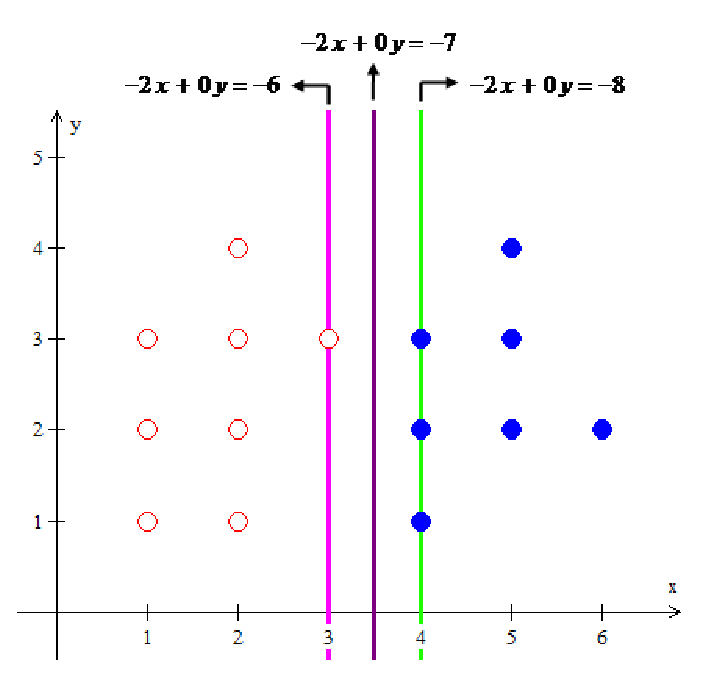
\includegraphics[scale=0.5]{graficos/exemplo2}
	\captionof{figure}{Representação ilustrativa do exemplo 1}
	\label{img:ex1}
\end{center}

A partir da representação gráfica podemos perceber que a reta separadora $-2x + 0y = -7$ se localizou exatamente no meio entre os dois conjuntos com o auxílio das duas retas: $-2x + 0y = -6$ e $-2x + 0y = -8$.

\item Exemplo2:
Vamos  considerar agora as matrizes:
$$A=\begin{bmatrix}3 & 4\\ 4.3 & 4.5\\ 4.5 & 2\\ 3 & 5.5\end{bmatrix}
B=\begin{bmatrix}4 & 2\\ 4.5 & 3.5\\ 5 & 3\end{bmatrix}$$

Neste exemplo temos: m = 4 e k = 3. De acordo com o modelo, temos os seguintes valores:
\begin{itemize}
\item[$\ast$] Valor da função objetivo = 0.92
\item[$\ast$] $\omega$ = [-0.91  0.91]
\item[$\ast$] $\gamma$ = -0.82
\item[$\ast$] y = [0 0 2.46 0]
\item[$\ast$] z = [0 0.91 0]
\end{itemize}

Com o valor da função objetivo diferente de zero, temos dois conjuntos linearmente inseparáveis, como ilustrado na figura a seguir.

\begin{center}
	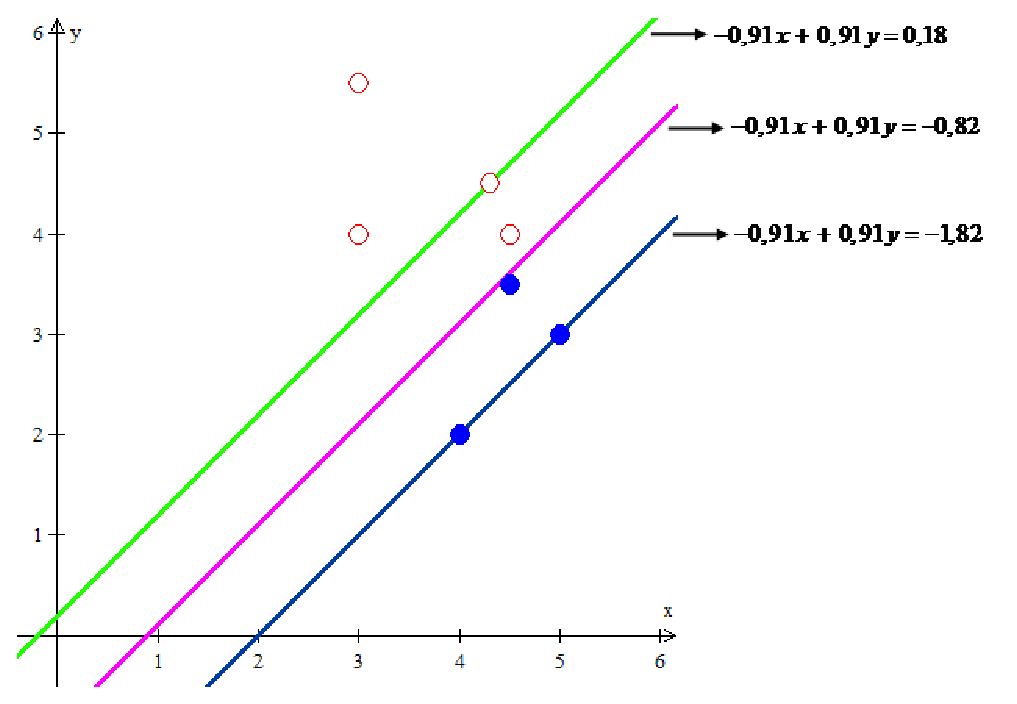
\includegraphics[scale=0.5]{graficos/exemplo1}
	\captionof{figure}{Representação ilustrativa do exemplo 2}
	\label{img:ex2}
\end{center}

Nesse exemplo notamos que o valor 2.46 no vetor y é referente ao ponto do conjunto A que está localizado do lado "errado" da reta. E o valor 0.91é referente ao ponto do conjunto B que está localizado mais próximo à reta separadora, apesar do ponto estar localizado do ponto correto da reta ele está localizado acima da reta limite $-0.91x + 0.91y = -1.82$. Concluindo que, quando um ponto está localizado do lado "correto" do hiperplano ou em cima de um dos hiperplanos limites, seu valor correspondente no vetor y ou z é nulo. Mas se um ponto está localizado do lado "errado" do hiperplano ou dentro da faixa formado pelos hiperplanos limites, seu valor correspondente no vetor y ou z é positivo.
\end{itemize}

\subsection{Geração de hiperplanos separadores}
Na etapa de treinamento, os padrões são agrupados em pares e dessa forma são submetidos ao modelo de programação linear, já que o modelo gera um hiperplano que separa dois padrões. Dessa forma para um conjunto de dados com N padrões, a quantidade de pares formados é dada pela fórmula:
$$ C_{N}^{2}=\frac{N!}{2\times (N-2)!)} $$

A etapa de treinamento consiste em gerar um hiperplano para cada par formado. No caso de um conjunto de dados constituido por 3 classes, são gerados 3 hiperplanos classificadores, da seguinte forma: 
\begin{figure}[h!]
\centering
\subfigure[Classificador dos padrões 1 e 2]{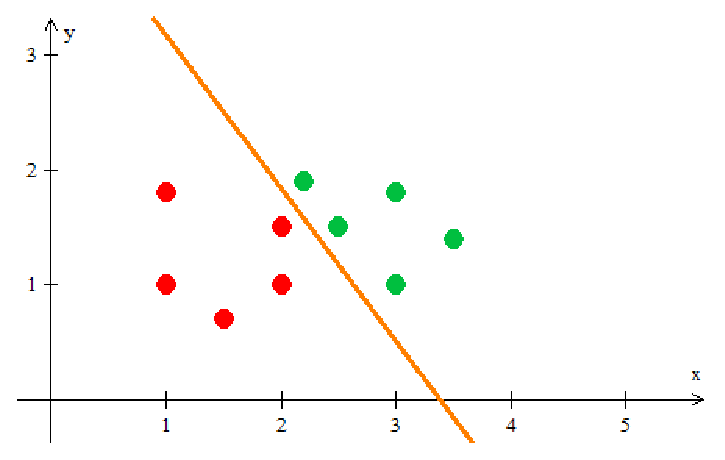
\includegraphics[scale=0.5]{graficos/class1e2}\label{fig1_ls}}
\qquad
\subfigure[Classificador dos padrões 1 e 3]{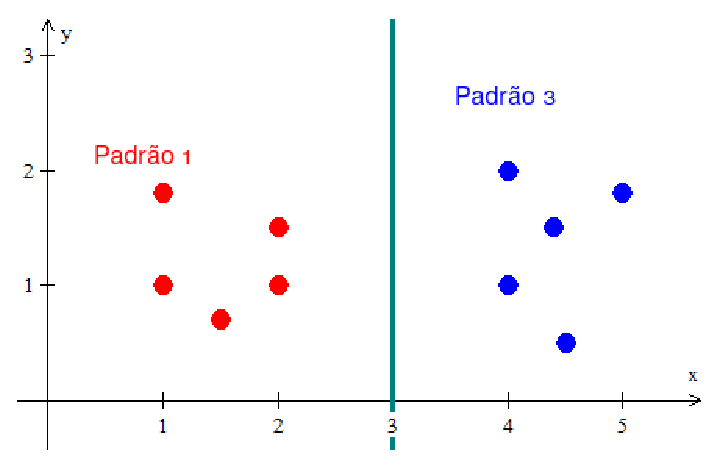
\includegraphics[scale=0.5]{graficos/class1e3}\label{fig2_ls}}
\qquad
\subfigure[Classificador dos padrões 2 e 3]{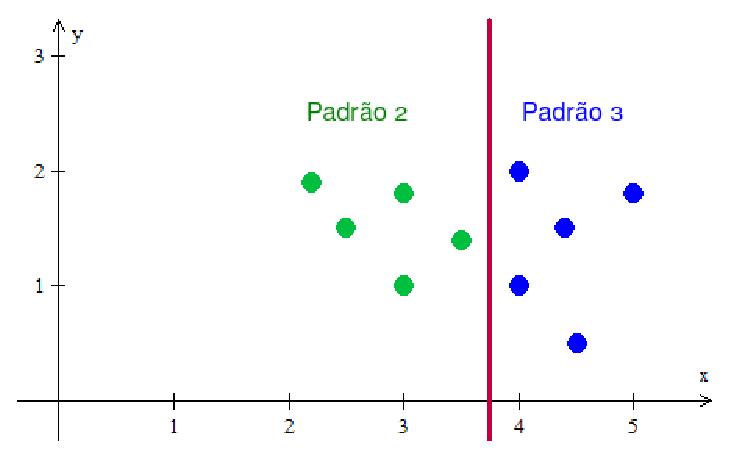
\includegraphics[scale=0.5]{graficos/class2e3}\label{fig3_ls}}
\label{img:linear_sepa}
\end{figure}

Na figura \ref{img:diagrama_modulos} o processo de treinamento corresponde ao módulo de geração de classificadores. Esse módulo foi implementado na linguagem de programação JAVA, utilizada como interface com o software CPLEX da IBM. O modelo é resolvido utilizando o método simplex revisado e toda etapa de resolução é feita pelo software CPLEX

\section{Etapa de classificação}
No processo de teste vetores de caracetrísticas são submetidos a estrtura de áravore de torneio e classificados em um dos N padrões do conjunto de dados.
Na figura \ref{img:diagrama_modulos} corresponde ao módulo de classificação de vetores com padrão desconhecido. E um arquivo contendo vários vetores para teste é utilizado.  A cada teste uma árvore de torneio é construída e um vetor para teste é lido e sua classificação é retornada. Na estrutura de árvore de torneio os padrões são confrontados aos pares, e o hiperplano que separa os dois padrões do par é utlizado para verificar de qual lado do hiperplano o vetor teste se localiza, o padrão que estiver do mesmo lado do vetor teste é elevado ao nível superior da árvore. Para verificar de qual lado o vetor teste de localiza é realizado o seguinte cálculo, considerando o vetor x como o vetor teste:

Se $ \begin{bmatrix}
\omega _{1} & ... & \omega _{n} 
\end{bmatrix}
\begin{bmatrix}
x_{1}
\\ 
.
\\
. 
\\
. 
\\
x_{n}
\end{bmatrix}
\geq \gamma $, o padrão A é elvado ao próximo nível da árvore;

Se $ \begin{bmatrix}
\omega _{1} & ... & \omega _{n} 
\end{bmatrix}
\begin{bmatrix}
x_{1}
\\ 
.
\\
. 
\\
. 
\\
x_{n}
\end{bmatrix}
\leq  \gamma $, o padrão B é elvado ao próximo nível da árvore.

Após a geração dos classificadores utlizando o modelo de programação linear, é necessário um segundo procedimento onde ocorra de fato classificação de um vetor com padrão inicialmente desconhecido. Nessa etapa de classificação foi implementada uma estrutura de árvore de torneio.
Em seus trabalhos \citeonline{Feng} e \citeonline{Guo} utilizaram a estrutura de árvore de torneio na etapa de classificação após a utilização do modelo de programação linear para gerar os classificadores.
A seguir são apresentadas duas figuras para ilustrar o mecanismo da árvore de torneio.

\begin{center}
	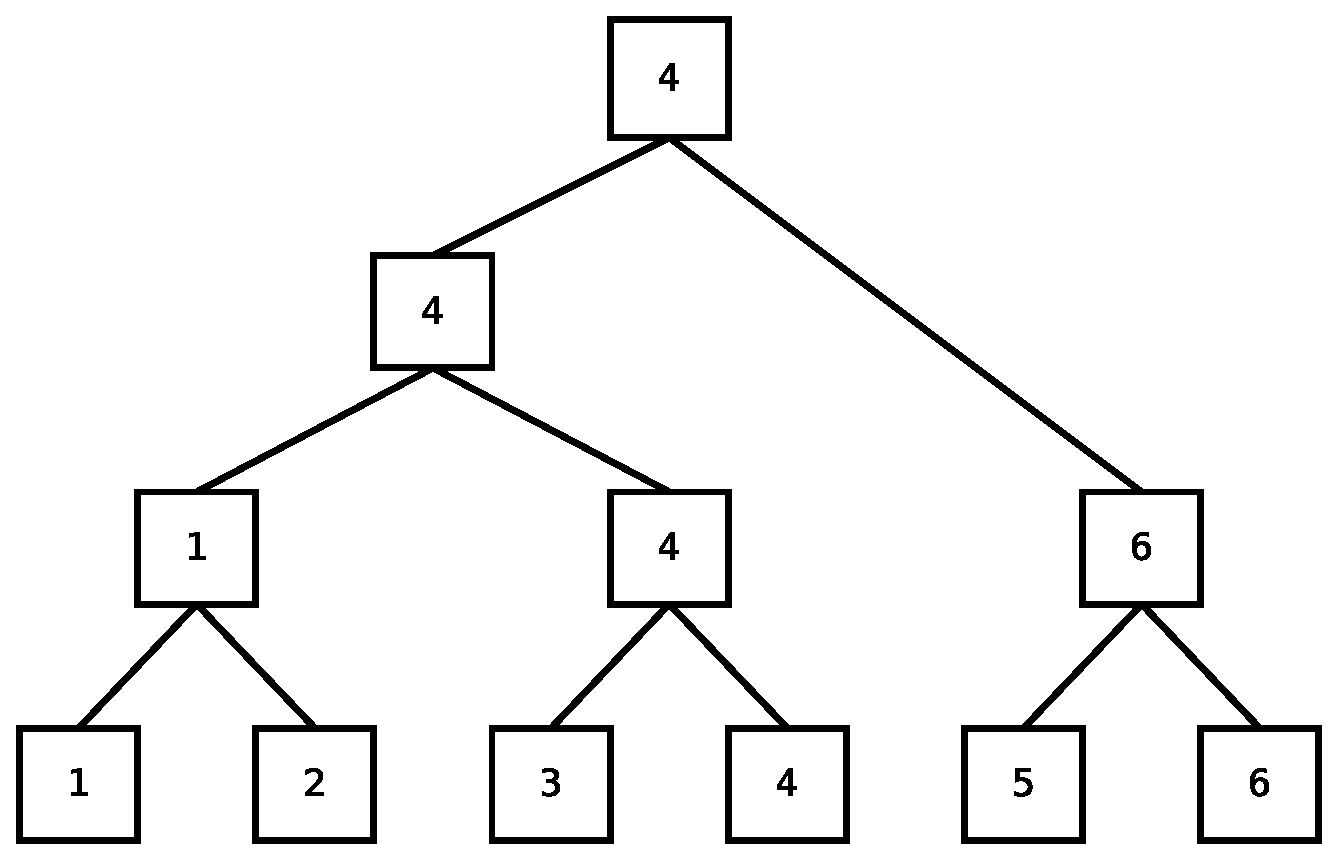
\includegraphics[scale=0.4]{graficos/ArvTorneio1}
	\captionof{figure}{Ilustração de uma árvore de torneio com 6 padrões}
	\label{img:ArvTorneio1}
\end{center}

\begin{center}
	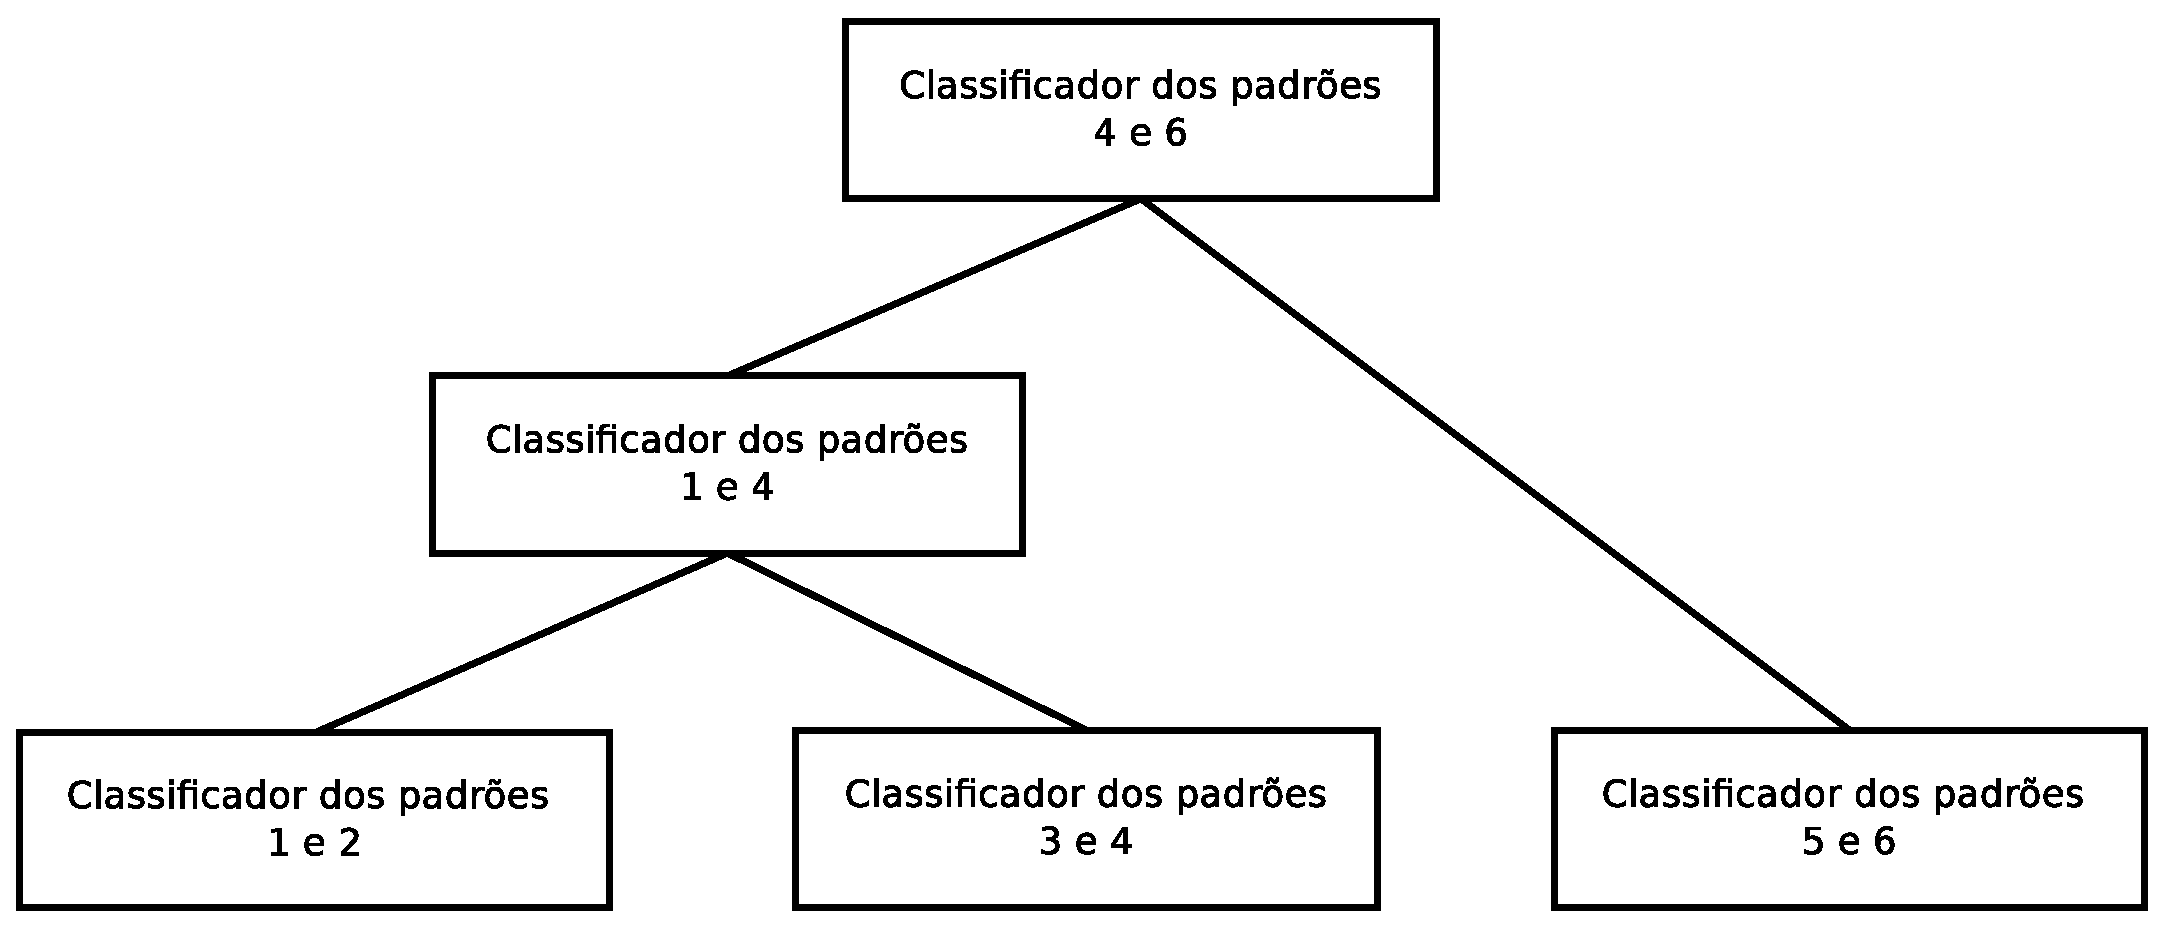
\includegraphics[scale=0.4]{graficos/ArvTorneio2}
	\captionof{figure}{Ilustração de uma árvore de torneio de acordo com os classificadores}
	\label{img:ArvTorneio2}
\end{center}
Depois de obtidos os hiperplanos separadores, é necessário um mecanismo para que um dado com padrão desconhecido possa ser classificado como um dos padrões, ou seja, analisando um vetor é preciso descobrir qual dos padrões ele se classifica. Para isso, é utilizada uma estrutura chamada árvore de torneio \cite{Feng} \cite{Guo}. Por analogia podemos pensar na árvore como a estrutura utilizada em um torneio esportivo e nos padrões como os times do torneio, os times devem se confrontar até que ao final saia o vencedor. Da mesma forma, analisamos os padrões até que ao final se obtenha o padrão ao qual o conjunto submetido pertença.
Na árvore da figura \ref{img:ArvTorneio1}, consideramos 6 padrões e o conjunto desconhecido pertencendo ao padrão 4. A quantidade de nós folhas deve ser a quantidade de padrões e a formação dos pares é arbitrária. Analisando o primeiro par, deve ser analisado em qual dos dois padrões o conjunto desconhecido mais se encaixa, ou seja, deve ser analisado de qual lado da reta (gerada pelo modelo quando foram submetidos os padrões 1 e 2, como ilustrado na figura \ref{img:ArvTorneio2})o conjunto desconhecido se encontra. Na figura exemplo, a maioria dos pontos ficaram localizados do mesmo lado da reta que os pontos do padrão 1, por isso esse padrão continuou no próximo nível da árvore e o padrão 2 foi excluído. Esse procedimento ocorre por analogia em todos os pares, até que ao final, quando analisados os padrões 4 e 6, foi definido que o vetor pertence ao padrão 4.

\subsection{Classificação com base em um hiperplano}
Dado um vetor x de caracteríticas, para determinar a qual padrão esse vetore pertence deve ser analisado de qual lado do hiperplano o ponto dado pelo vetor, se localiza, considerando que 
Se $ \begin{bmatrix}
\omega _{1} & ... & \omega _{n} 
\end{bmatrix}
\begin{bmatrix}
x_{1}
\\ 
.
\\
. 
\\
. 
\\
x_{n}
\end{bmatrix}
\geq \gamma $, x pertence ao padrão A;

Se $ \begin{bmatrix}
\omega _{1} & ... & \omega _{n} 
\end{bmatrix}
\begin{bmatrix}
x_{1}
\\ 
.
\\
. 
\\
. 
\\
x_{n}
\end{bmatrix}
\leq  \gamma $, x pertence ao padrão B.

Considerando o seguinte hiperplano em $R^{4}$:
$\omega$ = [1.21  8.0  -6.4  -19.2]
$\gamma$ = -33.6

E o vetor $x$ = [6.7  3.0  5.2  2.3], temos:

$ \begin{bmatrix}
1.21 & 8.0 & -6.4 & -19.2 
\end{bmatrix}
\begin{bmatrix}
6.7
\\ 
3.0
\\
5.2 
\\
2.3 
\end{bmatrix}
\leq  -33.6 $ 

Nesse caso o ponto representado pelo vetor x permaneceu do mesmo lado do hiperplano que os pontos do padrão B, sendo assim o vetor de caracteríticas x é reconhecido como pertencente ao padrão B. 

\subsection{Classificação com base na árvore binária de torneio}
Para o caso apresentado anteriormente foram considerados apenas dois padrões, porém em um problema que considera três ou mais padrões, é necessária a utlização de uma lógica para que seja realizado o reconhecimento do padrão entre \textit{p} padrões existentes. Nesse caso é utlizada a árvore binária de torneio.
Considerando um exemplo com três padrões (A, B e C), e os seguintes hiperplanos em $R^{4}$:
\begin{itemize}
\item Hiperplano separador dos padrões A e B
\subitem $\omega$ = [1.14  0.0  0.0  -7.86]
\subitem $\gamma$ = 0.0
\item Hiperplano separador dos padrões A e C
\subitem $\omega$ = [0.62  0.0  -1.03  0.0]
\subitem $\gamma$ = 0.0
\item Hiperplano separador dos padrões B e C
\subitem $\omega$ = [1.21  8.0  -6.4  -19.2]
\subitem $\gamma$ = -33.6
\end{itemize}

Para determinar a qual dos três padrões o vetor $x = [4.8  3.0  1.4  0.3]$, a árvore binária de torneio é montada dinâmicamente iniciando pelo nível de maior profundidade, nesse exemplo iniciamos com os padrões A e C.

\begin{center}
	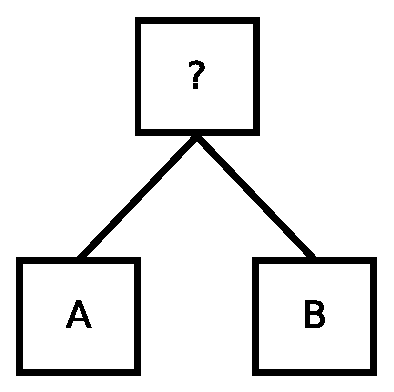
\includegraphics[scale=0.4]{graficos/arvore_nivel1}
	\captionof{figure}{Nós folhas no nível de maior profundidade}
	\label{img:Arv_nivel1}
\end{center}

Iniciando o reconhecimento do padrão do vetor x analisando os padrões A e B como ilustrado pela figura \ref{img:Arv_nivel1}, deve ser verificado de qual lado do hiperplano sepadarador dos padrões A e B o ponto representado pelo vetor x permanecerá
$ \begin{bmatrix}
4.8 & 3.0 & 1.4 & 0.3 
\end{bmatrix}
\begin{bmatrix}
1.14
\\ 
0.0
\\
0.0 
\\
-7.86 
\end{bmatrix}
\geq  0.0 $ 

Nessa primeira análise, o ponto representado pelo vetor x ficou localizado do mesmo lado do hiperplano que os pontos do padrão A. Então o padrão A é elevado ao próximo nível da árvore, como ilustrado na figura a seguir.

\begin{center}
	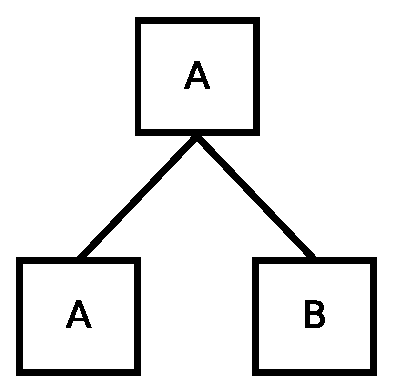
\includegraphics[scale=0.4]{graficos/arvore_nivel2}
	\captionof{figure}{Padrão A é elevado ao próximo nível da árvore}
	\label{img:Arv_nivel2}
\end{center}

Resta ainda analisar o padrão C.

\begin{center}
	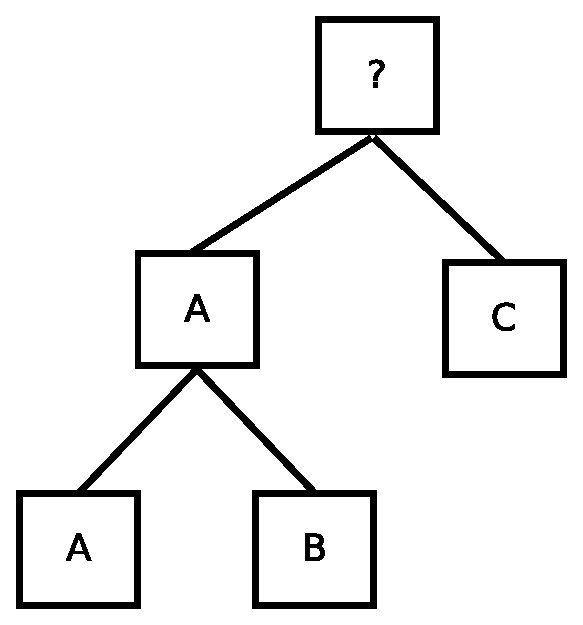
\includegraphics[scale=0.4]{graficos/arvore_nivel3}
	\captionof{figure}{Segundo nível da árvore}
	\label{img:Arv_nivel3}
\end{center}

Como mostrado na figura \ref{img:Arv_nivel3}, é feita a análise utilizando o hiperplano separador dor padrões A e C.
$ \begin{bmatrix}
4.8 & 3.0 & 1.4 & 0.3 
\end{bmatrix}
\begin{bmatrix}
0.62
\\ 
0.0
\\
-1.03
\\
0.0 
\end{bmatrix}
\geq  -33.6 $ 

Analisando o hiperplano separador dos padrões A e C é determinado que o ponto representado pelo vetor x ficou localizado do mesmo lado que os pontos do padrão A. Como todos os padrões (A, B e C) já foram analisados e a árvore foi completada, então, finalmente, o vetor x é reconhecido como pertencente ao padrão A.

\begin{center}
	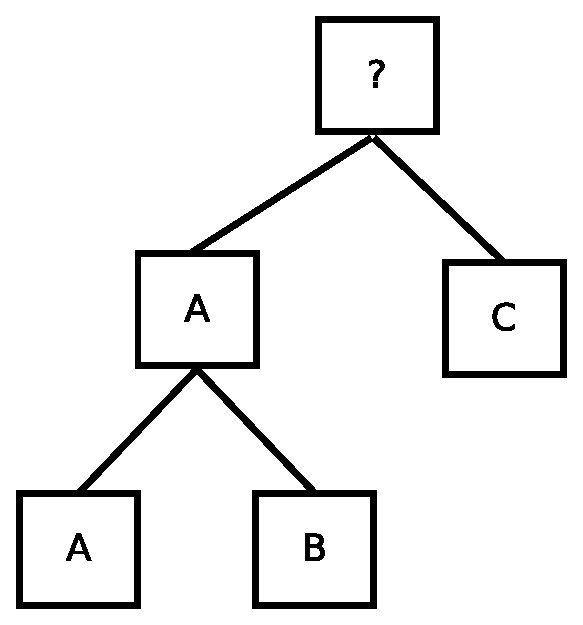
\includegraphics[scale=0.4]{graficos/arvore_nivel3}
	\captionof{figure}{Árvore completa}
	\label{img:Arv_completa}
\end{center}

A árvore completa é mostrada na figura \ref{img:Arv_completa}, após analisar todos os padrões, e o nó raiz da folha ser preenchido, a etapa de reconhecimento de padrão é completada, e o vetor com padrão inicialmente desconhecido é classificado como pertencente ao padrão que está no nó raíz da árvore.

\section{Etapa de validação}
Para testar a metodologia utlizada neste trabalho para o reconhecimento de padrões, foi utilizado o método cross validation \cite{Kohavi95Cross} \cite{Baldisserotto05Validacao}. Através dos resultados desse método é possível analisar a acurácia da metodologia de classificação, ou seja, a capacidade de classificar uma instância com o seu padrão correto.
Entre os três métodos de validação apresentados no referêncial teórico: Handout, Cross Validation e Leave One Out. O método cross validation foi escolhido como melhor opção já que os teste são feitos com vários conjuntos de dados com tamanhos variados. Para conjuntos de dados muito grandes o método Leave One Out se tornaria computacionalmete custoso e o método Handout poderia ter seu resultado comprometido de acordo com os parâmetros escolhidos na separação de dados para teste e de dados para validação. Além disso, o método Cross Validation é de fácil implementação e permite a utlização de todos os dados como teste e validação.
Na figura abaixo o método é ilustrado para o parâmetro 5 fold, apesar desse parâmetro não ter sido utlizado em nenhum teste, foi utlizado para um facilitar a ilustração. 
\begin{center}
	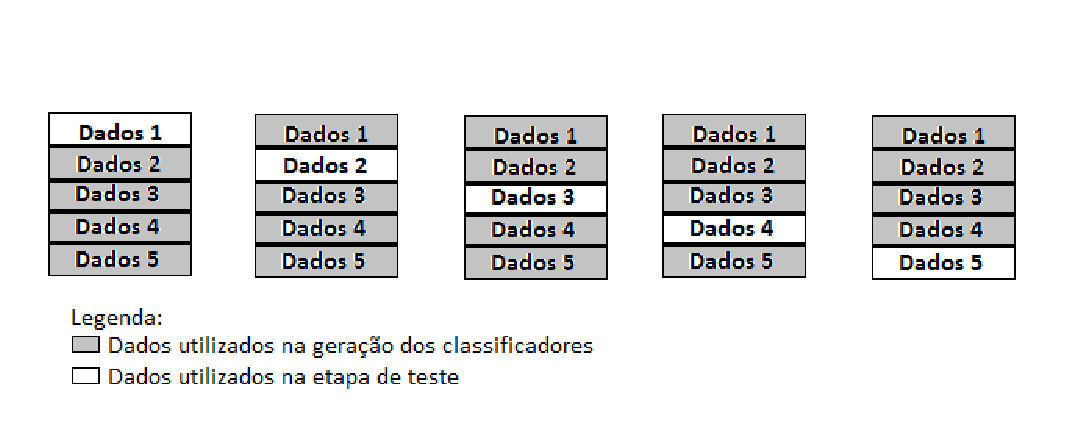
\includegraphics[scale=1.0]{graficos/cross_validation}
	\captionof{figure}{Mecanismo do método de validação 5-fold cross validation}
	\label{img:cross_validation}
\end{center}

Na ilustração o conjunto de dados foi dividido em 5 subconjuntos e consequentemente foram realizados 5 ciclos de treinamento e testes. A cada etapa 4 subconjuntos são utlizados para treinamento e um subconjunto diferente é utilizado para teste. 

A metodologia k-fold cross validation foi implementada na linguagem de programação Java. Os dados são organizados k arquivos. A implementação seleciona os dados de teste e de validação, e retorna o resultado parcial a cada rodada e o resultado final após os k ciclos de validação e teste. A cada ciclo de treinamento e teste a porcetagem de acerto de classificação é calculada da seguinte forma:

$$A = \frac{acertos}{total}\times 100$$

Onde total é a quantidade de vetores para classificação submetidos a cada ciclo de teste. E acertos é a quantidade de vetores que foram classificados corretamente.
